\documentclass{article}

% Language setting
% Replace `english' with e.g. `spanish' to change the document language
\usepackage[english]{babel}

% Set page size and margins
% Replace `letterpaper' with `a4paper' for UK/EU standard size
\usepackage[letterpaper,top=2cm,bottom=2cm,left=3cm,right=3cm,marginparwidth=1.75cm]{geometry}

% Useful packages
\usepackage{multicol}
\usepackage{amsmath}
\usepackage{graphicx}
\usepackage{array}
\usepackage{blindtext}
\usepackage[utf8]{inputenc}

\usepackage[colorlinks=true, allcolors=blue]{hyperref}

\title{POS Expression for Paper 2013 Question 6)c}
\author{Thoutu Rahul Raj}

\begin{document}
\begin{figure}
\maketitle
\begin{multicols}{2}
\tableofcontents
\vspace{10mm}

\begin{abstract}
 This manual shows how to use Arduino with LED to represent SOP expression for the function" X "shown in the  below truth table. \\
 
 \vspace{3mm}
 \centering
 
 \begin{tabular}{ |c |c |c |c |}
 \hline
 A  &  B  &  C  &  X\\
 \hline
 0  &  0  &  0  &  1\\
 \hline
 0  &  0  &  1  &  1\\
 \hline
 0  &  1  &  0  &  0\\
 \hline
 0  &  1  &  1  &  0\\
 \hline
 1  &  0  &  0  &  0\\
 \hline
 1  &  0  &  1  &  1\\
 \hline
 1  &  1  &  0  &  0\\
 \hline
 1  &  1  &  1  &  1\\
 \hline
 \end{tabular}
 \end{abstract}
 
\section{Components}

%\begin{table}[]
    \centering
    \begin{tabular}{ |c |c |c |c |}
\hline
\textbf{Components} & \textbf{Value} & \textbf{Quantity} \\
\hline
 %Resistor & 220Ohm & 1 \\ 
 Arduino & UNO & 1 \\  
 %Seven segment Display &  & 1 \\
 %Decoder& 7447&1 \\
 LED & - & 1 \\
 Jumper wires&M-M &3\\
 Breadboard& &1\\
 \hline
 \end{tabular}
 \vspace{3mm}
 
 %\caption{Table 1.0}
    %\label{table1}
%\end{table}

\section{Hardware}

\textbf{} Make connections between the Arduino and LED using Breadboard.

%\begin{figure}
 %    \centering
 %    \includegraphics{7447_pin.png}
  %   \includegraphics{7-Segment-Display-Pinout.jpg}
%\caption{7447 pin diagram}
 %    \label{fig:7447}
  %   \textbf{Problem 2.2}  Make connections to the lower pins of
%the 7447 according to Table 2.2 and connect VCC =
%5V. 
%\hfill
%\vspace{10mm}
%\includegraphics{7-Segment-Display-Pinout.jpg}
  %   \includegraphics{7-Segment-Display-Pinout.jpg}
%\caption{seven segment diagram}
 %    \label{fig:seven}
\section{Software}

\textbf{} Now make the connections as per
Table and execute the following program after
downloading.

\vspace{10mm}
\framebox{
\url{https://github.com/Rahulraj00/Assignments/Assignment 2}}

\vspace{10mm}
%\begin{table}[]
    \centering
    \begin{tabular}{ |c |c |c |c| c|}

%\textbf{Components} & \textbf{Value} & \textbf{Quantity} \\
\hline
 \textbf{LED}  & pin-1  & pin-2\\
 \hline
 \textbf{Arduino}  & 2 & GND\\  
 \hline
 \end{tabular}
 \vspace{3mm}
 
 %\caption{Table 1.0}
    %\label{table1}
%\end{table}


U, V, W are the
inputs and LED is the output.Using boolean
logic,
\begin{equation}
X=(!A\&\&!B)||(A\&\&C) 
%X = (!A&&!B) || (A&&C)
\end{equation} 
    \centering
    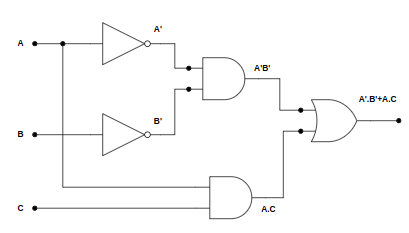
\includegraphics[width=\columnwidth]{assignment 2.png}
    \caption{logic diagram for A'.B'+A.B}    
\end{multicols}{}
\end{figure}
\end{document}

